\documentclass[sigconf]{acmart}

%%
%% \BibTeX command to typeset BibTeX logo in the docs
\AtBeginDocument{%
  \providecommand\BibTeX{{%
    Bib\TeX}}}

%% Rights management information.  This information is sent to you
%% when you complete the rights form.  These commands have SAMPLE
%% values in them; it is your responsibility as an author to replace
%% the commands and values with those provided to you when you
%% complete the rights form.
\setcopyright{acmcopyright}
\copyrightyear{2022}
\acmYear{2022}
\acmDOI{XXXXXXX.XXXXXXX}

%% These commands are for a PROCEEDINGS abstract or paper.
\acmConference[OCL 2022]{Make sure to enter the correct
  conference title from your rights confirmation emai}{October 23,
  2022}{Montreal, Canada}
\acmPrice{15.00}
\acmISBN{978-1-4503-XXXX-X/18/06}

%%\acmSubmissionID{123-A56-BU3}

%%
%% For managing citations, it is recommended to use bibliography
%% files in BibTeX format.
%%
%% You can then either use BibTeX with the ACM-Reference-Format style,
%% or BibLaTeX with the acmnumeric or acmauthoryear sytles, that include
%% support for advanced citation of software artefact from the
%% biblatex-software package, also separately available on CTAN.
%%
%% Look at the sample-*-biblatex.tex files for templates showcasing
%% the biblatex styles.
%%

%%
%% The majority of ACM publications use numbered citations and
%% references.  The command \citestyle{authoryear} switches to the
%% "author year" style.
%%
%% If you are preparing content for an event
%% sponsored by ACM SIGGRAPH, you must use the "author year" style of
%% citations and references.
%% Uncommenting
%% the next command will enable that style.
%%\citestyle{acmauthoryear}

\begin{document}

%%
%% The "title" command has an optional parameter,
%% allowing the author to define a "short title" to be used in page headers.
\title{Challenges for Code Generated OCL Execution}

%%
%% The "author" command and its associated commands are used to define
%% the authors and their affiliations.
%% Of note is the shared affiliation of the first two authors, and the
%% "authornote" and "authornotemark" commands
%% used to denote shared contribution to the research.
\author{Edward D. Willink}
\email{ed_at_willink.me.uk}
\affiliation{%
  \institution{Willink Transformations Ltd.}
%%  \streetaddress{P.O. Box 1212}
  \city{Reading}
  \state{Berks}
  \country{England}
%%  \postcode{43017-6221}
}

%%
%% By default, the full list of authors will be used in the page
%% headers. Often, this list is too long, and will overlap
%% other information printed in the page headers. This command allows
%% the author to define a more concise list
%% of authors' names for this purpose.
%%\renewcommand{\shortauthors}{Trovato et al.}

%%
%% The abstract is a short summary of the work to be presented in the
%% article.
\begin{abstract}
  While OCL is primarily a specification language supporting the elaboration of often-graphical metamodels with textual constraints, it is also executable enabling the constraints to be used to validate models. The superficial textual similarity of OCL and Java has tempted some authors to attempt a textual transliteration to facilitate a faster Java execution. Unfortunately there are many aspects of OCL semantics that deviate from Java and so transliteration is close to impossible. We identify the semantic differences so that new transliteration attempts can review the almost inevitable limitations of an OCL-like transliteration when choosing to implement a Java-Friendly OCL rather than a full OCL code generator.
\end{abstract}


%%
%% Keywords. The author(s) should pick words that accurately describe
%% the work being presented. Separate the keywords with commas.
\keywords{OCL, Code Generation, Optimization, Transliteration}
%% A "teaser" image appears between the author and affiliation
%% information and the body of the document, and typically spans the
%% page.
\begin{teaserfigure}
  \includegraphics[width=\textwidth]{OCLteaser.pdf}
  \caption{The OCL Compromise.}
  \Description{OCL wrt Java and Z.}
  \label{fig:teaser}
\end{teaserfigure}

%%
%% This command processes the author and affiliation and title
%% information and builds the first part of the formatted document.
\maketitle

\section{Introduction}
OCL is primarily a specification language supporting the elaboration
of often-graphical metamodels with textual constraints.

As shown in Figure~\ref{fig:teaser}, OCL\cite{OCL-2.4} compromises the familiar popularity of typical general purpose languages, such as Java, with formal languages, such as Z. Formal languages are so unfamiliar as to be unacceptable to many programmers. OCL's use, in conjunction with UML\cite{UML-2.5.1}, ensures that OCL has model oriented support. OCL's functional style facilitates a definition of a constraint as a compact expression.

The foregoing contrast is important but just ergonomic. More important for specification purposes is correctness, for which the generality of General Purpose Languages makes correctness proofs very hard if not impossible. In contrast, Formal Languages can be provably correct but the time and skills necessary to provide that proof are not available to many programmers or applications. OCL is positioned nicely between these two extremes. The relevant, accessible syntax means that 20 years on OCL is still the language of choice for writing model constraints. The potential for proof arises from the underlying side-effect-free functional specification principles. Sadly, the potential for proof has not been exploited and so remains just a potential for most specifications.

As a specification language, OCL is just a model-oriented pseudo-code, for which tooling ensures some degree of syntactic consistency with the standard. It is only once OCL's executable capability is realized that the pseudo-code is elevated to functional accuracy.

Model validation is an  important use case in which a model is loaded and all the applicable OCL constraints are executed to confirm that a model's Well Formedness Rules are respected. For large models, the efficiency of the execution is important and so it is attractive to replace a direct naive interpreted OCL execution of the WFRs by distinct compilation and execution phases. The compilation phase generates code in a language that can be executed faster.

In this paper, we first review the attraction of a transliterator in Section~\ref{Transliteration} and contrast it with the traditional tooling in Section~\ref{Tool Structure}. OCL and Java compatibility challenges are addressed in Section~\ref{Syntax Compatibility} for syntax and Section~\ref{Semantic Compatibility} for semantics. We then consider some code synthesis concerns in Section~\ref{Code Generation Synthesis} before summarizing the simplifications that a Java-Friendly OCL might make in Section~\ref{Java-Friendly OCL}. Related work follows in Section~\ref{Related Work} and we conclude in Section~\ref{Conclusion}. 

\section{Transliteration}\label{Transliteration}

Table~\ref{tab:Transliterations} shows examples of the kind of superficial textual and functional similarity between OCL and Java that have enticed some authors to attempt a textual transliteration.

\begin{table}
\begin{tabular}{ c | c }
 OCL & Similar Java \\
 \hline
 \hline
 name & name \\
 \hline
 (a = b) and true & (a == b) \&\& true \\
 \hline
 'xyzzy'.substring(a,b) & "xyzzy".substring(a,b) \\
 \hline
if a then b else c endif & if (a) \{ b \} else \{ c \} \\
\hline
 elements->forall(e : Element & for (Element e : elements) \\
 | body) & \{ body \} \\
 \hline
Set\{1, 1.0\}->size() & Sets.newHashSet(1, 1.0).size() \\
\end{tabular}
\caption{Alluring Transliterations}
\label{tab:Transliterations}
\end{table}

The examples in the table clearly show that neither character-by-character nor word-by-word transliteration is feasible. The challenge for a transliteration approach is to do sentence-by-sentence transliteration rather than a total analysis of the whole document followed by total synthesis by a code generator.

Unfortunately there are many aspects of OCL semantics that deviate from Java and so transliteration is close to impossible; there are too many concepts that require total analysis.

We briefly identify some errors in the alluring transliterations.

\verb|name| to \verb|name| is only correct if \verb|name| is the same concept in both languages. An unnavigable opposite would not be the same.

\verb|"xyzzy".substring(a,b)| neglects to correct from 1-based to 0-based indexes.

OCL's \verb|forall| is a multi-term \verb|and| operation whereas Java's \verb|for| does not relate its iterations. The transliteration should be more like:

\begin{verbatim}
boolean result = true;
for (Element e : elements) {
  if (!body) {
    result = false;
    break;
  }
}
... = result;
\end{verbatim} 

The \verb|Set{1, 1.0}->size()| demonstrates the uniformity of OCL numbers; the OCL size is 1 since OCL counts the number of distinct numeric DataType-typed  values. Java numbers are not uniform; the Java size is 2 since Java counts the number of distinct numeric Class-typed objects. A better transliteration could be

\begin{verbatim}
Sets.newHashSet(Double.valueOf(1), 1.0).size()
\end{verbatim} 

We revisit these and many other semantic differences so that a transliteration author can choose whether to resolve each difference by implementation heroism in the transliterator or by supporting a variant OCL subset that we refer to as Java-Friendly OCL (jfOCL).

% attempts can review the almost inevitable limitations of an OCL-like transliteration when choosing to implement a jfOCL2java rather than OCL2java code generator.

%elements->forall(hashValue.value = HashValue.value)
%children->forall(e : Element | e->collect(hashValue.value) = %self.oppositeOf(Parent::hashedValue).value)

% OSet numbers = H.equals()H.newOSet(H.newInteger(1), H.newReal(1.0)).size(), H.newInteger(1)

%We will now enumerate some of the significant issues that must be resolved during the CS to AS conversion.

\section{Tool Structure}\label{Tool Structure}

To understand what the transliterator does not do, it is helpful to review what standard tooling provides.

\subsection{Traditional Tooling Architecture}

\begin{figure}
	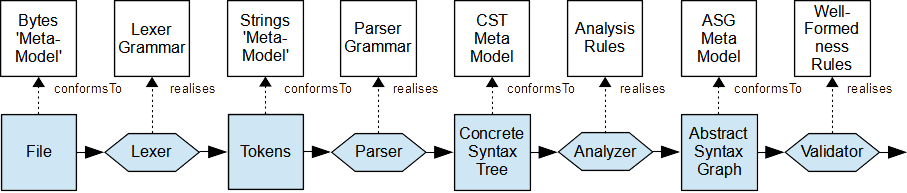
\includegraphics[width=3.0in]{OCLAnalysis.png}
	\caption{Traditional OCL Tool Architecture.}
	\Description{Traditional OCL Tool Architecture}
	\label{fig:parsing}
\end{figure}

The OCL specification separates concerns by suggesting an architecture such as Figure~\ref{fig:parsing} for an OCL tool.
%\begin{itemize}
%	\item convert (lex+parse) the source text to the Concrete Syntax
%	\item convert (analyze) the Concrete Syntax to the Abstract Syntax
%	\item execute (validate) the Abstract Syntax
%\end{itemize}

Lexer and Parser realize appropriate grammars to convert source file text characters via multi-character tokens to the Concrete Syntax Tree nodes.  

The Concrete Syntax provides a model that is close to the source text. Short forms are not elaborated. References are retained as unresolved names. The Concrete Syntax is therefore a Tree.

The Analyzer resolves the names to appropriate model elements, expands shortforms, synthesizes implicit iterators, elaborates implicit collect and infers types to annotate each node with accurate usage. A simple example for the OCL expression \verb|let c = a + b in ...| is shown in Figure~\ref{fig:exampleASG} using the style of a UML Object Diagram.

\begin{figure}
	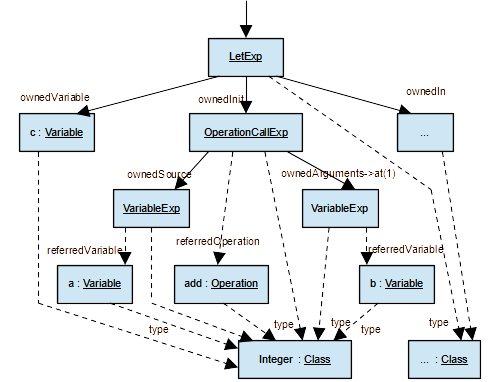
\includegraphics[width=3.0in]{OCLExampleASG.png}
	\caption{ASG of let c=a+b in ... example}
	\Description{ASG of let c=a+b in ... example}
	\label{fig:exampleASG}
\end{figure}

The composition tree has its root at the \verb|LetExp| node. It has an \verb|OperationCallExp| child and two further \verb|VariableExp| grandchildren. Composition is shown using directed solid edges between the nodes whose type is underlined. Additional references are shown as dashed edges. The \verb|referredOperation| identifies that \verb|OperationCallExp| executes using the \verb|Operation| named \verb|add|. Similar \verb|referredVariable| edges identify the variable to be read by each \verb|VariableExp|. The ancestry of the \verb|a| and \verb|b| variables and the \verb|Class| instances is not shown to avoid clutter. Nearly all the nodes in this simple example use the \verb|Integer| node as their \verb|type|. (The \verb|...| node and class are not relevant to this example; just necessary to make the \verb|LetExp| usage valid.)

The Abstract Syntax provides a rich model that is suitable for execution or further analysis. References are resolved unambiguously to model elements; the Abstract Syntax is therefore a Graph. 

The Validator is an example of a tool that executes the Abstract Syntax to determine whether a model confirms to its OCL-defined Well Formedness Rules. Execution typically uses an evaluator that interprets the ASG.

A Code Generator is another tool that can use the Abstract Syntax. It translates the ASG into a language that can execute more rapidly.

The existence of, and distance between, the CS and AS models is one of the major inconveniences for OCL tooling. The `draft'-like precision \cite{Willink2020} of the OCL specification is yet another major inconvenience requiring implementers to work hard to determine what was intended rather than specified.

\subsection{Transliterator Architecture}

\begin{figure}
	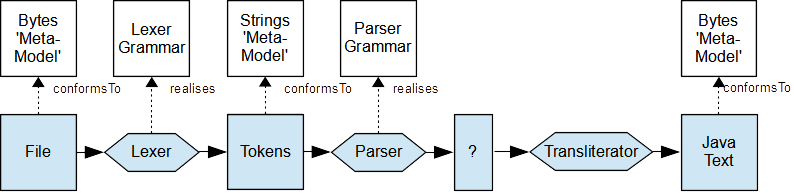
\includegraphics[width=3.0in]{Transliterator.png}
	\caption{Transliterator Architecture.}
	\Description{Transliterator Architecture}
	\label{fig:transliterator}
\end{figure}

An attraction of the transliterator is that it has a simpler tool architecture, as shown Figure~\ref{fig:transliterator}. The complexities of an Abstract Syntax are ignored; rather the transliterator comprises a simple serializer direct from the parser output to the required Java text. Ignoring the AS discards all the useful analysis that is captured in the AS. A transliterator author has just two choices. Either to replicate the analysis that underpins the AS, or to simplify the OCL language to such a degree that no analysis is needed.

\subsection{Evaluator Architecture}

While the Abstract Syntax is technically a graph, each OCL constraint is defined by an expression that is represented by a composition tree in which there is a child for each value needed to compute the result. Evaluation of an OCL expression is simply performed by a depth-first traversal of the composition tree. Once the traversal has reached the leaves, execution proceeds as each node returns its result to its parent.

If we consider the execution necessary for our simple example, whose OCL ASG is shown in Figure~\ref{fig:exampleASG}, we can see the execution cost of traversing the tree will far exceed that of the minimal pseudo-assembler for \verb|c=a+b|.

\begin{verbatim}
LD r0,a         -- load register r0 from memory a
LD r1,b         -- load register r1 from memory b
ADD r2,r0,r1    -- add r0 to r1 with result in r2
ST r2,c         -- store register r2 to memory c
\end{verbatim}

We might rate the pseudo-assembler as 25\% efficient since only one of the lines does necessary work; the other three control instructions shuffle values around memory and registers. In practice, we may achieve higher efficiency as the stores for a first expression may be rendered redundant with respect to the loads of a next expression. In the extreme case of a perfectly understood execution and unlimited registers, a near 100\% efficiency is possible. Of course a perfectly understood execution will give a very long entirely linear execution flow that need not actually execute at all; it can be optimized to return just the perfectly understood result.

Realistically, some control overhead is necessary for loops that accommodate data dependencies and reduce program size. A practical assembler implementation might perhaps aspire to 50\% efficiency.

If we now use a LISP-like assembler notation and consider the overheads of interpreting each opcode:
  
\begin{verbatim}
	(ST (ADD (LD a) (LD b)) c)
\end{verbatim}

There will be control overheads as each opcode such as LD is fetched and dispatched. Each nested term will result in a nested function call. It is easy to see that there are now many additional control overheads that are likely to reduce the efficiency well below 10\%.

A LISP-like selective rendering of the OCL ASG is even less direct

\begin{verbatim}
(LetExp #c
  (OperationCallExp "add"
    (VariableExp #a)
    (VariableExp #b)
  )
  ...
)
\end{verbatim}

After finding the \verb|OperationCallExp| opcode, the interpreter must fetch the \verb|"add"| argument and select the appropriate actions. This involves yet more control overheads so that the efficiency of interpreted OCL execution may well be only 1\%. This is clearly very disappointing and motivates the use of a code generator that can certainly do very much better than 1\%. At least 10\% should be possible using Java. Perhaps 25\% could be achieved using C as a portable assembler language. 

Perhaps the simplest approach to a speed up just provides a large library of helper functions for everything so that we may execute the Java serialization

\begin{verbatim}
doLetExp(env, "c", 
  doOperationCallExp_add(env, 
    doVariableExp(env, "a"),
    doVariableExp(env, "b"))
  )
);
\end{verbatim}

The above has already reified the \verb|"add"| into the operation-specific \verb|doOperationCallExp_add| helper, but has not reified \verb|"a"| as a variable; rather an \verb|env| is passed around. \verb|doVariableExp| may get from, and  \verb|doLetExp| may put to, the environment at a non-trivial cost. Clearly we can do better by exploiting Java variables directly, but we can start to see the challenges. Each change that we make to exploit a Java capability to realize an OCL capability must ensure that the Java execution observes OCL semantics. We will now examine the many ways in which OCL semantics differs from Java and why the following `obvious' Java is too simplistic.

\begin{verbatim}
int c = a + b;
\end{verbatim}

%\subsection{Code Generator Structure}

\section{Syntax Compatibility}\label{Syntax Compatibility}

We will first look at aspects of the OCL syntax that require accurate processing by the CS to AS analysis to determine the meaning. The code generator must faithfully represent the meaning as valid Java code. It is not clear how a transliterator can resolve the incompatibilities without the AS resolutions to guide the transliteration.

\subsection{Reserved Words}

Languages have reserved words that the user may not use as regular names. Use of a reserved word as a regular identifier almost always results in a compilation error that will prevent the transliterator being used. In pathological cases use of a reserved word could create a differently `valid' program.

In Essential OCL, names such as \verb|self|, \verb|else| and \verb|not| are reserved. In Complete OCL, names such as \verb|context| and \verb|package| are also reserved. \verb|forall| is not reserved. \verb|T| and \verb|T1| are also reserved but only to support the evasion of a proper implementation of UML templates. There is an escape mechanism so that \verb|_'\n'| or \verb|_'self'| may be used; any Unicode character sequence is an acceptable OCL name.

In Java, names such as \verb|this| and \verb|package| are reserved. There is no escape mechanism.

A transliteration of OCL to Java must therefore provide a mechanism to ensure a distinct and valid Java spelling for every possible OCL name spelling. jfOCL may attempt to push this responsibility back onto the OCL programmer, but sometimes metamodels have awkward names such as \verb|class|. Third party metamodels cannot be changed for the convenience of jfOCL.

\subsection{Shortforms, Name capture, Implicit Sources}

Object Oriented languages often allow a field of the current context object to be accessed without explicitly specifying the context object. Thus \texttt{self.name} in OCL, or \texttt{this.name} in Java can be shortened to just \texttt{name}. This is friendly but requires the transliterator to understand the OCL shorform before attempting to exploit a corresponding Java shorform.

\subsubsection{Java Shortforms}

In Java, \texttt{name} may refer to
\begin{itemize}
	\item a function parameter
	\item a local variable
	\item a non-static field of \texttt{this}
	\item a static field of \texttt{this.getClass()}
\end{itemize}
When there is only one option, user and tooling may be happy. When there is an unresolvable ambiguity, tooling must report a compilation error. But sometimes there is a resolution priority; a function parameter hides a non-static field. This priority may not always suit the user, so tooling may offer a warning to encourage the user to rename the parameter and so avoid the hazard.

Further complexity arises when an outer definition may be accessed from within
\begin{itemize}
	\item a nested class
	\item an anonymous function
	\item a lambda.
\end{itemize}

\subsubsection{OCL Shortforms}

OCL's name resolution policies are similar

\begin{itemize}
	\item an operation parameter
	\item a let variable
	\item a non-static property of \texttt{self}
	\item a static property of \texttt{self.oclType()}
\end{itemize}
but include 
\begin{itemize}
	\item any unique iterator
	\item an advanced navigation
	\item a type
	\item a template parameter
\end{itemize}

\paragraph{Implicit Sources}
The OCL implicit iterator source is dangerously flexible. In

\begin{verbatim}
books->forall(b
             | chapters->forall(c
                               | authors->notEmpty()))
\end{verbatim}

\verb|authors| can be a shortform for \verb|c.authors| or \verb|b.authors| or \verb|self.authors| or a let-variable or a function parameter. The iterator shortform is a candidate even when the explicit \verb|b| and \verb|c| iterators are implicit. Resolution of the shortform requires a search of the metamodel to see whether \verb|Chapter::authors| or \verb|Book::authors| exist before considering the usual candidates. jfOCL might well prohibit the dangerous nested implicit source. Prohibiting the immediate loop iterator could be a step too far.  

\paragraph{OCL Navigation}
%\subsection{Opposite Navigation}

%The ability to navigate a unidirectional association in the reverse direction through the implicit opposite syntax provides a powerful ability for OCL constraints to apply to unhelpful metamodels. Unfortunately, as well as analysis challenges, an evaluation is obliged to  perform a near-total model search to locate the opposite. A good implementation can avoid incurring this cost more than once.

In addition to the traditional Object Oriented instance to slot interpretation of the dot navigation operator, OCL normalizes a variety of different forms of navigation behind the one syntax. The most complicated is probably the implicit opposite navigation for which the transliterator must generate a call to an appropriate helper that searches the model for the required opposite. See Section~\ref{Properties}  and Section~\ref{Implicit Opposites} for further details.

\paragraph{OCL Type Names}

OCL lacks a distinctive type literal syntax analogous to Java's \texttt{MyClass.class}. Consequently the argument for \texttt{oclIsKindOf(V)} may refer to the type \texttt{V} or the property \texttt{V} or the let-variable \texttt{V} or ...

OCL is UML-aligned, consequently OCL supports UML templates even though the OCL specification lacks any grammar, concrete or abstract syntax support. Once templates are  supported, template parameters are yet another option for a name reference.

\subsubsection{Summary}

The many differences in name resolution make it unsafe to attempt to transliterate shortforms directly from OCL to Java. The actual access must be understood, matched to an appropriate Java access, and then serialized in a way that ensures that the appropriate access is actually used.

\section{Semantic Compatibility}\label{Semantic Compatibility}

Once the OCL semantics has been identified, it is possible to translate the OCL into Java that exhibits the identical OCL semantics. We must therefore identify how and when OCL semantics can be realized in Java. Generating Java without an appropriate understanding risks generating inaccurate code. We will therefore examine the compatibility of various constructs.

\subsection{Program Structure}
	
Java package, class and operation constructs are very similar and more powerful than OCL's so there is little difficulty in using mapping OCL structural concepts to a subset of Java.

\subsection{Properties}\label{Properties}

OCL, or rather UML or Ecore, has Classes with Properties in a similar fashion to Java's Classes with Fields, so it would seem that the \verb|aY.x| OCL navigation using the unidirectional association from \verb|Y| to \verb|X| in Figure~\ref{fig:navigation} can be transliterated to \verb|aY.x| in Java.

But this is to ignore the power of OCL's model oriented support. OCL supports many different forms of Property navigation, many of which appear to be simple.

Even the simplest access may need care since OCL does not specify the reification of each class instance. Distinct mechanisms will probably be needed depending whether the source and/or target class instance is:
\begin{itemize}
	\item Java Object
	\item Java Bean
	\item EMF EObject
	\item XML Element
	\item Object Data Base Object
	\item UML Instance
	\item UML Stereotype
	\item UML Association
\end{itemize} 

The transliterator must invoke an appropriate helper, since direct use of Java's mechanism is not often correct. Distinct mechanisms will usually be needed depending whether the access is to DataType of Class object and whether the access is to a single object or a collection of objects.

\begin{figure}
	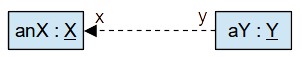
\includegraphics[width=2.0in]{OCLOpposite.png}
	\caption{Navigation example}
	\Description{Navigation example}
	\label{fig:navigation}
\end{figure}

OCL hides a variety of access mechanisms behind the simple dot-navigation syntax. The implicit opposite syntax is useful and powerful but hard to implement. With respect to Figure~\ref{fig:navigation}, OCL supports the \verb|anX.y| navigation even though \verb|X::y| is not navigable. Implementation of this is discussed in Section \ref{Implicit Opposites}.
(Further lexical complexities arise when the \verb|y| role is omitted from the metamodel. A default name is available by re-using the name of the target type allowing \verb|anX.Y|. If the auto-generated name is ambiguous the more elaborate \verb|anX.Y[Y::x]| syntax may be used.) 

Yet more complexity arises from

\begin{itemize}
	\item static properties
	\item derived properties
	\item inherited properties
	\item Stereotype  properties
	\item Association-owned properties
	\item UML subset/union/redefined properties
\end{itemize} 

Access to a property is only part of the challenge. Many properties may have an OCL expression defining the initial and/or derived value that must be calculated in a timely fashion and which may need to be cached to avoid redundant calculation. But once cached, the external usage must be respected to invalidate the cache in an equally timely fashion.

It is not clear how this can be done without an overall analysis to determine all the forms of property access that occur, then to plan an implementation strategy, and finally to synthesize distinct construction code as well as the use of an appropriate helper for the actual access.

\subsection{Control Semantics}

OCL's operation call and return is broadly compatible with Java.

OCL's \verb|if then else endif| is easily accommodated in Java.

An OCL let-variable is relatively easily realized by a Java variable declaration.

OCL's loops do not have direct Java counterparts, so helpers or templates are required. See Section~\ref{Loop Synthesis}.

There is a major incompatibility in regard to OCL's \verb|invalid| which is philosophically the same as a Java exception but very different implementation-wise.
\texttt{invalid} handles the very inconvenient use case where the program flow fails perhaps due to a program error, perhaps due to an external environment problem.

OCL's \texttt{invalid} is a value that is returned as an alternative to the intended value and must be propagated through every computation until it is handled or returned as the overall result.

In contrast, a Java exception is a \texttt{Throwable} instance that is thrown. It bypasses all intermediate computations until a catch handler is encountered.

These very different practical semantics are not amenable to naive transliteration.

An implementation may chose to use Java exception semantics throughout the transliteration. Every generation of an OCL \texttt{invalid} must then be replaced by a thrown \texttt{Throwable}. Conversely every OCL operation that may be passed an \texttt{invalid} value must have an operation call that carefully catches any exceptions to create the required \texttt{invalid}. This is inconvenient for ordinary code, it is distinctly awkward when the exception can occur while initializing a let variable.

Alternatively, an implementation may use OCL \texttt{invalid} semantics throughout the transliteration. This then requires every helper to be accurately coded to guarantee that exceptions are returned as \texttt{invalid}, a guarantee that is likely to be overlooked by maintainers. Every call to a helper may therefore need to wrapped in an exception conversion. All helpers must be coded to propagate \texttt{invalid}.

The latter approach could be suitable if \texttt{invalid} was a prolific use case, but hopefully \texttt{invalid} is rare, so it is more efficient to work with, rather than against, Java's natural capabilities. It is appropriate to analyze the potentially invalid flows in order to plan the necessary catch handlers. An accurate analysis can ensure that only those very rare let-variables that can propagate an invalid value incur the overheads.

Implementation of \texttt{invalid} is a significant pain, so tools may follow USE's\cite{USE} example and omit support for \texttt{invalid} altogether. However this is not OCL; it provides support only for OCL programs that never fail. There will be no divide-by-zero, no null-navigation, no index-out-of-bounds on ordered collections.

None of the above approaches is attractive. Careful study of the OCL specification reveals that it is well-intentioned but irrational~\cite{Willink2021}. A much more practical and sensible design can be compatible with Java exception semantics. Unavoidable exceptions such as a network-failure are classified as desirable exceptions that should always be thrown. Programming errors such as collection-index-out-of-bounds are classified as undesirable exceptions that should be eliminated by analysis at compile time. The challenging need for commutative rather than short-circuit \verb|and|/\verb|or| operators that uncrash can be eliminated by commuting the inputs at compile time to guarantee that only the second input can crash.

The OCL validity analysis \cite{Willink2021} is a non-trivial whole program analysis that cannot possibly be done sentence-by-sentence. However the motivation of the analysis is to prove that the OCL is free of undesirable crashes. jfOCL could define all crashes as desirable avoiding the need to catch any exceptions anywhere. It is only necessary to convert \texttt{invalid} to a thrown exception. This is easily done by providing no reification of \texttt{invalid}; exceptions can be thrown from the outset. With no catching of exceptions, a rational implementation of \verb|and|/\verb|or| that computes first argument first will exhibit the familiar short-circuit behaviour.

\subsection{Type / Value}

When we use helper functions to implement each OCL semantic, the values we pass to the functions and which are returned by those functions should observe OCL semantics and conform to OCL types.

Before we examine typical types, we should note one important difference between OCL/UML and Java. UML defines two kinds of Object, Class-typed and DataType-typed. A Class is instantiated as an instance which typically has a unique address and so two distinct class instances are not equal. A DataType defines a value that is often embedded as the attribute of an instance. A DataType does not have a unique address. DataType values are equal when a deep comparison of their information fields finds all are equal.

Java has user-defined Class instances but only built-in primitive DataType values. There is a flexibility to overload \verb|equals()| so that, for instance, a pair of \verb|String| instances can compare equal even when their addresses differ. This is important to avoid the need for \verb|Map| keys to be used without the overhead of interning. This can lead to some surprises whenever \verb|int|, \verb|double|, \verb|Integer| and \verb|Double| are intermixed.
The surprise is demonstrated by the difficulty in transliterating \verb|Set{1, 1.0}->size()| to ensure that the two representations of the one value populate a single-entry Set.

The overt example mixing real and integer literals is perhaps unrealistic so jfOCL could prohibit it. More complex examples might not be apparent to the user, so jfOCL should diagnose them, however the effort required to diagnose them is comparable to the effort required to enforce the common type determined by the regular OCL analysis. jfOCL should really support numeric value uniformity.

\subsubsection{Boolean, String}

The semantics of Boolean and String values are compatible so Java's type and values can be used. Only a little care is needed where the spelling of operations such as \verb|toUpper| varies.

\subsubsection{UnlimitedNatural}

Java has no counterpart to UnlimitedNatural, so a helper type is necessary. However UnlimitedNatural is not a numeric type, rather it is an unbounded enumeration used solely to support the upperbound of UML's Multiplicity. jfOCL might omit UnlimitedNatural.

\subsubsection{Integer, Numeric Precision}

OCL specifies two ideal numeric types \texttt{Real} and \texttt{Integer}, whereas Java specifies many practical types such as \texttt{int}, \texttt{Long} and \texttt{BigInteger} with inconsistently imperfect functionality. A 32 bit integer is sufficient for almost all use cases, but just occasionally position or time calculations need more.

Suppose your salary is represented by a 32 bit integer. Given severe inflation and a persistently generous boss, your salary may grow to the 31 bit threshold. If you are `lucky', your salary may saturate. If `unlucky', a wraparound occurs to negative numbers and you have to pay to work. 

This is disappointing but OK in Java; it is what the specification says should happen. It is absolutely not OK in OCL for which unbounded integers grow and grow.

An OCL2Java conversion must choose a Java representation for OCL's \texttt{Integer}
\begin{itemize}
	\item always 32 bit Integer
	\item always 64 bit Long
	\item always BigInteger
	\item use a variety of types
\end{itemize}

32 bits is simple and efficient but significantly defective.

64 bits is simple and similarly efficient on a modern 64 bit machine and very rarely defective.

BigInteger is costly for the vast majority of use cases and defective only in pathologically huge use cases.

The approach taken by the pivot-based Eclipse OCL is to use a polymorphic abstract \texttt{IntegerValue}, It has \texttt{LongIntegerValue},\\ \texttt{IntIntegerValue} and \texttt{BigIntegerValue} concrete derived classes. The implementation of addition returns a larger type when required.

\texttt{IntIntegerValue} like Java's \texttt{Integer} wraps an underlying \texttt{int} content so there is very little performance penalty for the `correct' solution.

\subsubsection{Real}

Floating point arithmetic is little used in OCL, so there is little benefit in struggling to use \verb|Float| or \verb|Double| rather than \verb|BigDecimal| everywhere.

\subsubsection{Object}

References to Model Elements can be compatible. Conversely, if they are not, the overheads of converting or wrapping Objects incur an undesirable cost.

\subsubsection{Collection}

Java's Collection types were originally designed as non-template types. These were upgraded to templated classes when Java 5 added generics, but backward compatibility necessitated a concept of type erasure. This means that the actual templating type is not known at run-time preventing expressions such as \verb|new T()|.

OCL's collection types have a magic \verb|T| that behaves in many ways like a template parameter. Once the requirement for UML alignment is respected, the magic \verb|T| can be respecified as a regular template parameter and the rules for collection type conformance revisited to avoid the anomaly that \verb|Set{}->including(4)| is erroneous. The empty \verb|Set{}| is a \verb|Set(OclVoid)|. When the source argument is used to specialize the \verb|Set(T)::including(T)| operation to \verb|Set(OclVoid)::including(OclVoid)| the error arises because \verb|4| does not conform to \verb|OclVoid|. More declaratively, there is an alternative specialization \verb|Set(Integer)::including(Integer)| for which both source and argument are type conformant.

Eclipse OCL applies this declarative philosophy to ensure that the Abstract Syntax is annotated with consistent specializations. The \verb|Operation::type| declaration has the unspecialized type. The invoking \verb|OperationCallExp::type| has the specialized type. 
These types are propagated and checked throughout the AST. They provide the accuracy necessary to declare variables in Java and to inject the necessary casts from what the OCL analysis guarantees to what the Java declarations require.

%Despite its specified alignment with UML that has templated types, the OCL specification neglects to provide any grammar, modeling or rules for templates. Complying with the UML alignment aspect is therefore entirely down to the enthusiasm of the OCL vendor. This enthusiasm may extend to resolving the conformance of templates types so as to avoid \verb|Set{}->including(4)| being a type conformance error, since an \verb|Integer| cannot be added to the empty \verb|Set(OclVoid)|. The OCL Standard library provides the operation \verb|Set(T)->including(T)| for which \verb|Set(Integer)->including(Integer)| is a suitable specialization. It is not clear from the current specification whether \verb|C1(T1)| conforms to \verb|C2(T2)| when \verb|T1| conforms to \verb|T2| and \verb|C1| conforms to \verb|C2|. OCL can have a good specification of templates without being hampered by a non-template legacy.

%Resolution of template specializations is an important part of the OCL analysis type checking. The results are persisted in the OCL AST. An OperationCallExp.referredOperation .type provides the unspecialized return type of the declaration, OperationCallExp.type gives the corresponding specialized type.

The Java \verb|Set<T>| and OCL \verb|Set(T)| classes are templated so that the programmer can enforce their intent. A \verb|SetValue| class that provides the underlying implementation of \verb|Set(T)| for OCL does not need to be a templated class since the underlying implementation can access the template parameter more flexibly as a regular field rather than as a template parameter. 

Unless jfOCL replicates the collection type analysis, the transliterator may have to sprinkle the code with casts of dubious validity.

Java provides \verb|ArrayList| and \verb|HashSet| that can be used relatively easily to implement OCL's \verb|Sequence| and \verb|Set| collections. \verb|LinkedHashSet| can be used for \verb|OrderedSet| once a bug-fixing \verb|equals| overload is provided to ensure that differently-ordered contents are not equal. There is no Java counterpart for \verb|Bag|. jfOCL can exclude \verb|Bag| or provide a custom helper type.

\subsubsection{Compatible Value Representation}

One of the many challenges in implementing an OCL tool is the lack of a specification of the surrounding environment. OCL is an add-on to an existing system with which OCL must co-exist. There may therefore be three distinct representations of the same value. So considering a Set of Integer and EMF as an example surrounding environment, the usage may need to be

\begin{itemize}
	\item SetValue for use in OCL support helpers
	\item Set<BigInteger> when interacting with a Java routine
	\item EList<EInt> when interacting with EMF
\end{itemize}

The transliterator must track the prevailing representation of each passed value and invoke conversions whenever necessary.

\subsubsection{Conformance, Inheritance, OclAny, OclVoid}\label{Conformance}

OCL supports type conformance whereas Java supports single-class, multiple-interface inheritance.

For most types conformance and inheritance are the same, but OCL adds a conformance from all classes to \texttt{OclAny} and from \texttt{OclVoid} to all classes.

UML\cite{UML-2.0} (and Ecore) metamodels may use multiple-class inheritance. The EMF\cite{Eclipse-EMF} support uses distinct interface and implementation classes so that the interfaces accurately model the multiple inheritance. The implementation classes can only inherit one implementation and so the auto-generation re-implements all additional inheritances to create the illusion of true multiple-class inheritance.

Helper functions for OCL conformance cannot rely on Java's reflection capabilities so custom metadata may be required.

jfOCL may choose to prohibit multiple inheritance and not support OclAny or OclVoid.

\subsection{Null}

OCL's \texttt{null} is very similar to \texttt{null} in Java.

Difficulties can arise if the implementation of a type such as an enumeration fails to provide for a null value,

\subsection{Operation}

A distinct Java function can be provided for every OCL operation. This makes it more likely that OCL semantics are used throughout, but incurs a significant coding effort. It is therefore desirable to use pre-existing Java implementations wherever possible with the occasional wrapper to ensure appropriate semantics.

There are however some notable function/operation inconsistencies.

\subsubsection{Boolean Short-Circuiting}

Many languages provide a short-circuit capability for Boolean operations whereby in, for instance \verb|a && b|, no attempt to evaluate \texttt{b} occurs if \texttt{a} is false. If evaluation of \texttt{a} crashes, the overall evaluation crashes.

OCL specifies commutative Boolean operations, which allows the OCL evaluation of \verb|a and b| to evaluate its inputs in any order or concurrently. If the earliest input evaluation crashes and is \texttt{invalid}, but then the later input evaluation is \texttt{false}, the crash of the earlier term is `uncrashed'.

This very different semantics prohibits the simple transliteration of \texttt{and} to \texttt{\&\&}. A helper operation can support the OCL-and semantics in Java. Since the helper requires \texttt{invalid} input values, the caller must ensure that any Java exceptions are caught.

The OCL validity analysis \cite{Willink2021} enables the inconvenient commutated short circuit use case to be detected and rewritten so that regular Java exception semantics can be used.

\subsubsection{Indexes}

Java follows the tradition of implementation languages with arrays and lists using 0-based indexes. Conversely OCL follows the specification tradition of 1-based indexes. Java operations that take an index argument have an easily resolved semantic incompatibility.
The transliterator must convert the index base at some point taking care to convert exactly once.

\subsubsection{Implicit Operations}

OCL uses dot navigation for object navigation and arrow navigation for collections. Additionally, OCL defines an arrow navigation for objects that is equivalent to an invocation of \verb|oclAsSet| and a dot navigation for collections that is equivalent to invocation of a \verb|collect()| iteration. These implicit invocations are expanded by the OCL analyzer as it creates the AS. A transliterator that ignores the AS must replicate the analysis that in some cases must accurately resolve types to distinguish whether for instance \verb|myAggregate.name| is an implicit collect of a user collection type or a simple navigation of a regular class.

Java does not (yet) have null-safe navigation and so an implementation of OCL that provides null-safe operators \cite{Willink2015} must again replicate the synthesis that the analyzer performs when synthesizing the ASG.  

\subsection{OCL-specific}

Some OCL concepts have no direct Java counterpart.

\subsubsection{Tuple}

In Java a primary type such as \verb|MyClass<T>| is declared once. Its specialization such as \verb|MyClass<String>| may be `declared' many times with each re-`declaration' sharing  the same specialized type.

OCL does not declare types at all; types are declared elsewhere in some metamodel. Usage of the collection types such as \verb|Bag(String)| behave in a very similar way to a Java specialization, perhaps confirming that the magic \verb|T| that parameterizes them should be modeled as a UML TemplateParameter.

An OCL Tuple type has no unique declaration, rather each repetition of the same  set of \{name,type\} pairs is the same type. Java has no corresponding dynamically constructed type, so a code generator must pre-analyze the OCL to aggregate all Tuple declarations and create a conventional Java class for each distinct Tuple type.

Alternatively jfOCL may prohibit Tuples.

\subsubsection{oclIsKindOf(), oclType(), reflection}

As noted in Section~\ref{Conformance} OCL uses conformance rather than inheritance and while the concepts are similar there are subtle differences that \texttt{oclIsKindOf()} and \texttt{oclIsTypeOf()} must respect.

OCL's \texttt{oclIsKindOf()} is similar to \texttt{instanceof} in Java, and
\texttt{oclType()} is similar to Java's \texttt{getClass()} however they operate on different type systems. The OCL calls use modeled types where Java uses Java classes. Sometimes these are the same, but more often they differ. In Ecore there is typically a distinct interface and implementation Java class for each modeled class. Any multiple inheritance in the model is respected by the interfaces but only emulated by the classes.

Helper functions for \texttt{oclIsKindOf()} and \texttt{oclType()} must respect the OCL type conformance relationships. An implementation can provide tables to facilitate efficient access. These tables may support full reflective capabilities rather than the very partial form specified for \texttt{oclType()}.

\subsubsection{oclIsNew() and @pre}

OCL's \texttt{oclIsNew()} and OCL's \texttt{@pre} may only be used in post-conditions in order to contrast the system state on entry and exit states of an operation. This has no counterpart in Java and implementation of a helper is hard.

This is a difficult corner of the OCL specification that jfOCL may reasonably choose to skip.

Eclipse OCL\cite{Eclipse-OCL} with an emphasis on execution has no execution capability for \texttt{oclIsNew()} or \texttt{@pre}. No user has ever complained.

USE\cite{USE} has an emphasis on simulation and a custom model framework that supports a `filmstrip'~\cite{Desai} of system states. This is able to support \texttt{oclIsNew()} and \texttt{@pre}.

In principle, the support for two system states, may require the operation entry code to have a complete copy of the system state. This can be difficult and expensive, but is only necessary when the post-condition's \texttt{@pre} access involves a cascade of collection operations that are too complex to analyze. In practice, the \texttt{@pre} accesses are often trivial making an on-entry copy simple.

\subsection{Model / UML-specific}

OCL provides some unique capabilities associated with its support for models.

\subsubsection{allInstances()}

OCL's \texttt{allInstances()} has no counterpart in Java. The deficiency can be remedied by a helper function that traverses the transitive closure of the containment and reference relationships starting from a single seed model element. This assumes that the Java objects have sufficient context to reflect on the metamodels that define the Java classes. EMF provides this capability.

%This limitation, like many other problems can be side-stepped by delegating the problem to a helper function; the synthesized code just makes a suitably parameterized call to the relevant helper.

%Implementation of the helper requires access to all the model objects. This is hard in Java, but straightforward when a framework such as EMF supervises model elements.

A naive helper implementation may perform a total model search for every \texttt{allInstances()} call. A better implementation may start with a metamodel analysis of the OCL to determine the typically small number of calls that can occur followed by a model analysis to determine all required \texttt{allInstances()} in one model traversal. This may be performed as part of the initial model loading or lazily when the first call occurs.

\subsubsection{Implicit Opposites}\label{Implicit Opposites}

OCL's opposite navigation again has no counterpart in Java and like \texttt{allInstances()} can be remedied by a helper function that traverses the whole model searching for the solutions. Again, like \texttt{allInstances()}, a naive implementation may be very costly, but a better implementation may use a metamodel analysis to discover all the \verb|X::y| unnavigable opposites actually in use so that a single traversal of the model can populate a cache of \verb|{X -> X::y}| for constant-time cost during execution. These analyses can be performed at the same time as the \texttt{allInstances()} search.

\subsubsection{Stereotype}

Normal OCL usage involves developing a typically M1 metamodel that constrains the corresponding M0 instances. OCL constraints are written against the metamodel and evaluated on the model.

UML Stereotypes provide a confusing ability to merge extensions into the M1 metamodel classes. The extensions are defined in the M2 metametamodel. OCL constraints are written against the metametamodel and evaluated on the M1 metamodel to verify consistent extension usage.

When a Stereotype provides an additional property \verb|P::p|, it is accessed by an M2 constraint as \verb|aY.extension_P.p|. However at M0, the Stereotype is logically folded into the extended instance and so the access may be \verb|aY.p|. How this folding actually occurs is dependent on the model support. For EMF-based UML2Ecore, the properties are folded in as regular properties subject to spelling adjustments to avoid clashes. For UML, the run-time is a little vague, but probably the property is not folded, rather the missing StereotypeApplication metaclass that lies behind the XMI magic, needs to be reified to support accessing the stereotype application as a sub-object. Whatever, the transliterator must choose and parameterize an appropriate helper to perform the property access.

\section{Code Generation Synthesis}\label{Code Generation Synthesis}

We have identified the near-impossibility of a sentence-by-sentence transliteration and so we now describe a few synthesis considerations for a code generator. The code generator uses the Abstract Syntax Graph as input and so has an accurate representation of what needs to be done; all intermediate expression types are known, synthetic operations such as safe navigation and implicit collect have been elaborated, implicit iterator variables have been created and names resolved appropriately. 

\subsection{Name Synthesis}

The initial implementations of new tools are rarely bug free, consequently users as well as developers may need to study the generated code to understand what has gone wrong, and perhaps to find a workaround for a bug. This study is eased if the code is pleasantly formatted and if the names are easily related to names that are already familiar to the user.

Mindless re-use of names from metamodels and OCL can fail through use of reserved words, multiple use of the same name or differential name occlusion between Java and OCL.

These failures can be resolved by accurately tracking the names visible in each synthesis scope and generating names that avoid clashes. The user's names can provide hints to which prefixes or suffixes are applied to clarify roles and avoid clashes.

%Readability important to accommodate bad abstraction.

%When OCL is code generated as Java, the resulting Java can be made more readable if the name of an element in the OCL is re-used in the Java. This is clearly not possible when the OCL name is a Java reserved word such as \texttt{package}. The reserved word clash can be resolved by a name mangling convention but there is a risk that the mangled name then clashes with another name. More generally the same name may be used for multiple purposes in OCL, but the same re-uses my lead to an ambiguity in Java.

%The Java synthesis must accurately track the scopes of all name usages to ensure that clashes are replaced by distinct unique names. The original OCL names can be used as hints for their Java names; they cannot be used directly.

\subsection{Loop Synthesis}\label{Loop Synthesis}

It was noted in Table~\ref{tab:Simplifications} that while OCL's \verb|forall| looks rather like Java's \verb|for|, a more complex text template is needed. The following text template can be used for iterations other than \verb|closure()| that merits a dedicated handler. 
\\
\verb||\textit{declare-result}\verb|;|\\
\verb|{|\\
\verb|    |\textit{declare-and-initialize-iterator(s)}\verb|;|\\
\verb|    |\textit{declare-and-initialize-accumulator}\verb|;|\\
\verb|    while (true) {|\\
\verb|        if (|\textit{iteration-done}\verb|) {|\\
\verb|        	|\textit{assign-result-from-final-accumulator-value}\verb|;|\\
\verb|        	break;|\\
\verb|        }|\\
\verb|        |\textit{advance-iterator(s)}\verb|;|\\
\verb|        |\textit{execute-iteration-body-and-assign-to-accumulator}\verb|;|\\
\verb|    }|\\
\verb|}|

For the common single iterator iterations, it is well worth generating inline Java to reduce control overheads. For less common iterations such as \verb|sortedBy| or multi-dimensional iterations, it may be appropriate to realize the text template by virtual function calls to a polymorphic loop manager and to pass the body as an anonymous function.

\subsection{Code Generator Model and Optimization}

The Abstract Syntax Graph is a good model of the OCL semantics, but somewhat distant from the Java semantics. A Code Generator may therefore choose to transform the OCL ASG into a more Object-Oriented Code Generator Model from which generation of Java or C or ... is much easier. In the ASG, every expression term can return a value. In the CGM, every not-inlined expression term may return a Static Single Assignment variable facilitating a synthesis that can always refer to a variable. The expression terms include many extra terms to cast to known types, guard against nulls and convert between representations. The substantial support code to provide conformance tables, or implicit opposite caches can be reified in the CGM reducing the complexity of the eventual CGM to text model-to-text transformation. (For Eclipse OCL a further CGM to JavaModel to JavaText intermediate is planned.) 

Once a sensible CGM is in use, support for optimizations such as Common Subexpression Elimination, Constant Folding and Loop Hoisting follows naturally. The Validity Analysis ~\cite{Willink2021} is a significant extension to Constant Folding that once integrated should identify many more candidates for Dead Code Elimination.

\section{Java-Friendly OCL}\label{Java-Friendly OCL}

While describing the various challenges, we have identified deviations from specified OCL that a hypothetical jfOCL might adopt in order to avoid the complexity of a full OCL analysis and subsequent synthesis.

A potential OCL tool vendor may reasonably ask why it is so hard to develop OCL tools. We have provided some of the answers

\begin{itemize}
	\item poor quality of the specification
	\item lack of standard surrounding model access
	\item subtly distinct semantics from Java
\end{itemize}

Unfortunately a jfOCL only addresses some of the distinct semantics.

\begin{table}
\begin{tabular}{ c | c | c }
Concept & Eclipse OCL & jfOCL \\
\hline
iterator shortforms & supported & prohibited \\
Java reserved words & supported & prohibited \\
\hline
invalid & supported & crash always \\
Bag & supported & prohibited \\
Integer/Real & polymorphic & distinct \\
OclAny & supported & prohibited \\
OclVoid & supported & prohibited \\
UnlimitedNatural & supported & prohibited \\
oclIsKindOf() & supported & prohibited \\
oclType() & supported & prohibited \\
and/or & commutative & short-circuit \\
\hline
allInstances() & supported & prohibited \\
implicit opposites & supported & prohibited \\
qualified navigation & supported & prohibited \\
qualified associations & supported & prohibited \\
qualified navigation & supported & prohibited \\
Tuples & supported & prohibited \\
\hline
%associations & partially supported & not supported \\
stereotypes & supported & not supported \\
@pre, oclIsNew() & not supported & prohibited \\
\end{tabular}
\caption{Simplification Options}
\label{tab:Simplifications}
\end{table}

Each of the simplifications summarized in Table~\ref{tab:Simplifications} enables a jfOCL to be more like Java making the jfOCL2java transliteration easier, but if too many are adopted there must be a question as to whether too much of OCL has been discarded. Many of the original advantages of OCL such as compact collection cascades and iterations have been diminished by the advent of Java streams and lambdas. Perhaps it would be better to devote the development effort to providing a better library of helpers for regular Java use and possibly some annotation magic to facilitate model-oriented use.

Revisiting Figure~\ref{fig:teaser}, the outstanding advantage of OCL is its potential for provable correctness. Discarding too much of OCL may not only reduce the richness but also undermine the correctness. Once this happens, OCL becomes pointless.

\section{Related Work}\label{Related Work}

This paper revisits Willink~\cite{Willink2012} in which "An extensible OCL Virtual Machine and Code Generator" was presented. It probably remains as the only extensible code generator for `full' OCL (and QVTc and QVTr). Ten years on, the emphasis on a VM is clearly misleading hype. A VM suggests a JVM-like byte code interpreter, which is possible, but something of a premature optimization. The XMI serialization of the OCL ASG is more appropriate. Compacting it to byte code while saving on file size would needlessly lose readability when debugging. In this paper we draw on 10 years evolution to explain why a `full' code generator is hard so that other authors tempted to develop one can fully appreciate the challenges they face.

Many authors have provided a partial OCL code generator demonstrating good characteristics aligned with some research goal. Omission of OCL facilities such as oclIsNew(), @pre,  allInstances(), States, Messages and even Tuples and opposites is common, but in many cases this just represents a pragmatic reduction of scope to facilitate research; these omissions can be rectified by a little more work. Failure to address unbounded numerics, numeric equality, null/invalid propagation, nested Collections and oclType() is a more fundamental challenge to some of the approaches. 

Wilke\cite{Dresden/JavaCG} describes a reworked  Java generator for Dresden OCL based on parameterized fragments.
AspectJ is used to support model access in Java models. However many Java types are used directly and so functionality is limited to Java-like semantics for numeric range and equality.

Heidenreich\cite{QueryCode} describes a Dresden OCL generator for SQL based on identifying typical patterns of database usage. It is not clear that this is able to handle arbitrary OCL or OCL that fails to exhibit SQL-like characteristics.

Egea\cite{MySQL4OCL} describes a MySQL generator to avoid the heavy overhead of loading a large model into an OCL tool. Stored procedures are used to realize the iterations that are common to many typical applications. The procedures are then executed within an SQL database. This is an interesting deployment option but does not help with full-functionality OCL code generation.

Shidqie\cite{Shidqie} introduces Imperative Ecore as an intermediate model to separate OCL restructuring and Java formatting concerns, but ignores non-Java-like aspects such as unbounded numbers.

Moiseev\cite{rodion-models2009} takes a more progressive transformational approach realized as rewrites in Maude. This is clearly beneficial when supporting multiple target languages, unfortunately it ignores the awkward aspects of OCL.

%Mezei\cite{OCL-relocation} relocates and caches OCL evaluations to reduce navigation costs.

More recently Lano\cite{Lano2021} has used some powerful rules to create a remarkably small transliterator from OCL to Swift. It is not clear how this approach avoids the need for an overall analysis, how extensive the library of helpers is, or how the reference and ambiguity resolution of a traditional OCL analyzer is replicated. 

\section{Conclusion}\label{Conclusion}

We have identified how the `friendliness' of OCL's shortforms requires significant semantic analysis to enable an appropriate exposition in the semantics of another language.

Since the results of this analysis are available in the OCL Abstract Syntax, we conclude that synthesis of code from the semantically resolved AS can be accurate. In contrast, full transliteration is only possible if the standard CS to AS conversion is duplicated within the transliterator.

We have enumerated many of the OCL facilities such as opposite-navigation, unbounded-integers and invalid that are inconvenient to code generate so that OCL-like implementers can determine which inconveniences to omit in their `Java-Friendly OCL'.

%%
%% The next two lines define the bibliography style to be used, and
%% the bibliography file.
\bibliographystyle{ACM-Reference-Format}
\bibliography{OCLCodeGeneration}

\end{document}
\endinput
